%!TEX root = ../../main.tex

\chapter{Silicon Vacancy Centers in Diamond}	\label{ch::sivs}
\chaptermark{SiV Centers}

\begin{remark}
    \begin{itemize}
      \item test
    \end{itemize}
\end{remark}

\section{Diamond as a host lattice}

  Diamond is a metastable modification of carbon which is, in fact, stable under normal conditions \cite{steinmetz::52}. Carbon atoms form strong $sp3$-bonds with each other in a tetraedal arrangement of neighboring atoms. The resulting $sp3$-hybridized lattice is of exceptional mechanical stability, making diamond the hardest known material \cite{?}. The crystal structure can also be interpreted as a face-centered cubic (fcc) lattice with two carbon atoms in the primitive Bravais cell, situated at $(0,0,0) \ a$ and $ (\frac{1}{4}, \frac{1}{4}, \frac{1}{4}) \ a$ with $a = \SI{3.567}{\angstrom}$ denoting the lattice constant \cite{steinmetz::56}. \autoref{fig::diamond_lattice} illustrates the structure.

  \begin{figure}[htp]
		\centering
		\testbox{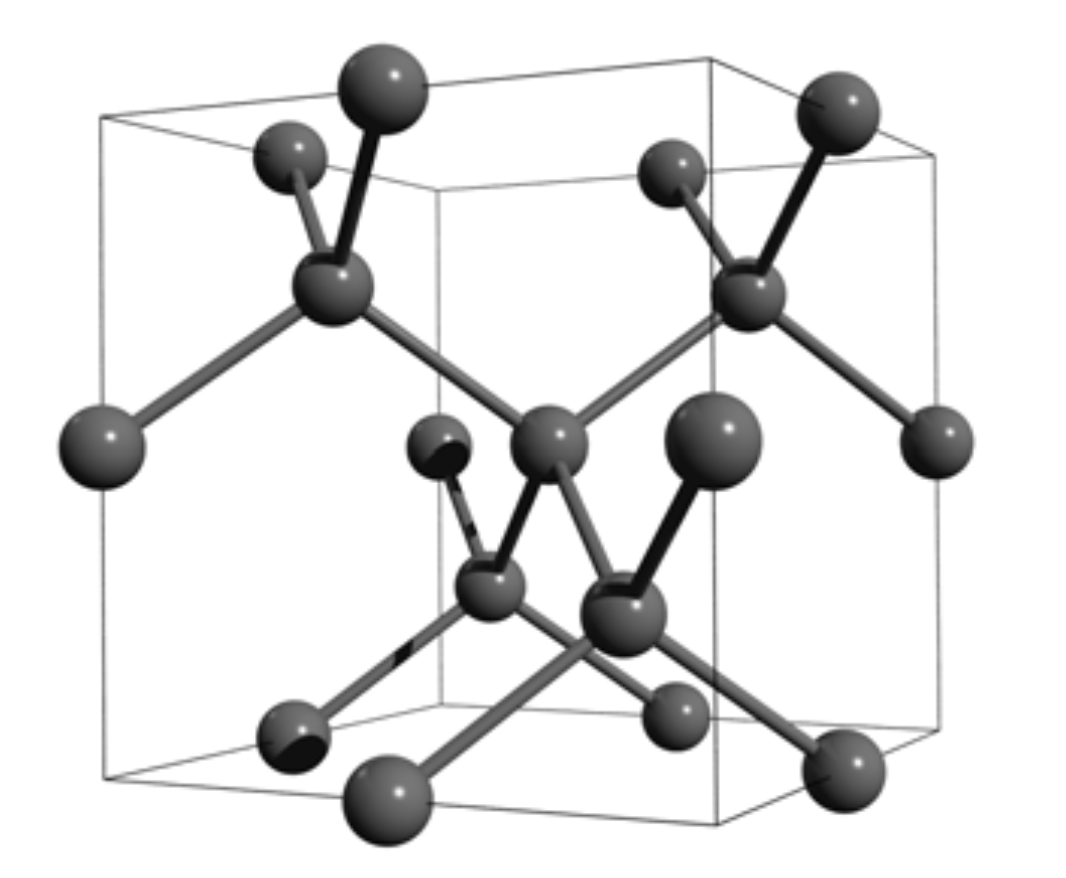
\includegraphics[trim = 0 0 0 0,  clip= true, width = 0.3\textwidth]{./pics/diamond_lattice.png}}
		\caption{Face-cendered cubic diamond lattice. Note the tetraedal arrangements of carbon atoms. Figure reproduced with permission from \cite{janine::thesis}.}
		\label{fig::diamond_lattice}
	\end{figure}

  The valence and conduction bands of diamond are separated energetically by a large direct band gap of \SI{7.3}{\eV} while its indirect band gap amounts to \SI{5.5}{\eV} \cite{steinmetz::57, neu::91}. As a result diamonds are transparent for light of all wavelengths larger than \SI{230}{\nm} \cite{neu::87}. This transparent quality makes diamond an ideal host material for various optically active lattice defects or impurities. These induce a wide range of discrete energy levels accomodated by the sizable band gap. The absorption of optically active impurities or impurity complexes gives rise to the color of diamonds, thus these impurities are commonly termed color centers \cite{neu::thesis}. Due to the exceptional mechanical stability of diamond color centers too are very stable, another important property enabling optical applications.

  A property of diamond, detremental to some optical applications, is its large refractive index with values of $2.49$ at \SI{360}{\nm} and $2.4$ at \SI{800}{\nm} respectively \cite{steinmetz::58}. Thus, a portion of the flourescent light escaping from the diamond is reflected back into it, effectively reducing the efficiency of light extraction. If \nds smaller than the wavelenght of the light to be collected are used, internal reflection is supressed and the extraction efficiency can be increased \cite{neu::49}.

  \begin{figure}[htp]
		\centering
		\testbox{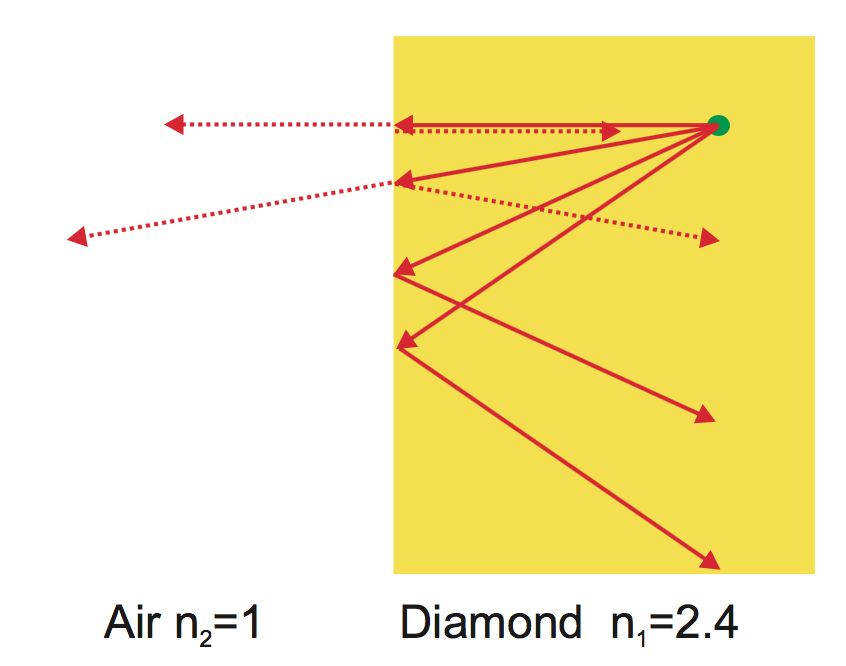
\includegraphics[trim = 0 0 0 0, clip= true, width = 0.3\textwidth]{./pics/diamond_refraction.png}}
		\caption{Light from a flourescent emmitter inside the diamond (green dot) undergoes reflection at the diamond-air interface. Figure reproduced with permission from \cite{neu::thesis}.}
		\label{fig::diamond_refraction}
	\end{figure}

  \subsection{Types of diamonds}

    Two major approches for classifying diamond are commonly encountered. First, classification according to the presence or absence of certain impurities or impurity complexes. Second, classification based on different diamond crystallinities observed. In the following both classification systems are briefly introduced.

    \subsubsection{Classification by impurities}

      Impurities or complexes of impurities in the diamond lattice can be optically active and thus change the optical properties of diamond. Most strikingly perhaps is the appearence of color in otherwise colorless diamond due to a sufficient concentration of such defects. Using IR absorption spectroscopy the degree of nitrogen impurtities can be determined. It is used to subdivide diamonds into distinct groups named Type I and Type II \cite{janine::148, janine::149}. The groups are further subdivided as follows:

      \begin{itemize}
            \item Type Ia: With a nitrogen concentration of up to \SI{3000}{ppm} most natural occuring diamonds belong to this group \cite{steinmetz::58}. Nitrogen appears arranged predominantly in aggregate clusters forming complexes of impurties. These complexes are optically active, absorbing light in the blue range of the visible spectrum. Consequently Type Ia diamonds often exhibit a yellow to brownish coloration.

            \item Type Ib: With concentrations of up to \SI{500}{ppm} nitrogen atoms appear predominantly in isolation, replacing individual carbon atoms in the diamond lattice. In addition to absorbing visible blue light, green is being absorbed as well. Type Ib diamond thus exibits intensified the yellow or brownish coloration. While only \SI{0.1}{\percent} of naturally occuring diamond fall into this class, almost all synthetic diamonds created using the high-pressure-high-temperature method are of Type Ib \cite{steinmetz::58}.
      \end{itemize}

      While Type I diamond exhibits an appreciable concentration of nitrogen, Type II diamonds lack nitrogen entirely. Type II diamond is divided into two subgroups according to the presence or absence of boron as follows:

      \begin{itemize}
        \item Type IIa: Can be considered pure as they lack boron impurities and other optically active defects \cite{neu::84}. They thus are colorless. Up to \SI{2}{\percent} of natrually occuring diamond and most diamonds synthetically created using the chemical vapor deposition method are of Type IIa \cite{steinmetz::58}.
        \item Type IIb: Contains appreciable concentrations of boron atoms replacing individual carbon atoms in the diamond lattice. Boron defects are optically active absorbing visible light ranging from red to yellow. Depending on the Boron concentration blue to grey colorations are observed. Furthermore, diamond is turned from an insulator to a efficient p-type semiconductor in the presence of boron impurities \cite{steinmetz::59}.
      \end{itemize}

      We remark that for many modern applications of diamonds the presented ``classic" categorisation of diamond is not enough. Thus a precise quantification of the concentration and nature of various relevant impurities is often called-for. In this section we also briefly touched upon two methods to synthetically produce diamonds. Both are relevant for this thesis and are explained in detail in \autoref{ch::fabrication_nanodiamonds}.

    \subsubsection{Classification by morphology}

      %steinmetz
      Da es im späteren Verlauf dieser Arbeit auch Diamantproben einer anderen Mor- phologie als der einkristallinen betrachtet werden, soll kurz auf die unterschiedlichen Formen von CVD-Diamanten eingegangen werden. Bei deren Herstellung spielen so- wohl die Wachstumsparameter als auch die Art des verwendeten Substrates eine wichtige Rolle, da entsprechende Veränderungen die Morphologie der hergestellten Schichten deutlich verändern können. So ist es zur Herstellung eines Einkristalls not- wendig, ein Substrat zu verwenden, dessen Gitterparameter möglichst gut mit denen des zu wachsenden Diamanten übereinstimmen. Dies betrifft zum einen Gitterkon- stante (3,57Å) und -struktur (fcc mit zweiatomiger Basis), als auch den niedrigen thermischen Ausdehnungskoeffizienten des Diamanten von ca. 0,7 × 10−6 K−1 bei Raumtemperatur [61]. Das nächstliegende Substrat ist Diamant selbst [62] – man spricht in einem solchen Fall von Homoepitaxie. So kann man z.B. einen mit dem HPHT-Verfahren hergestellten und damit weniger reiner Stein als Substrat für einen reineren CVD-Diamanten verwenden, der dann nach dem Wachstum beispielsweise durch Laserschneiden von dem Substrat gelöst wird. Inzwischen ist es jedoch ebenfalls gelungen, Diamant auf fremde Substrate zu wachsen. Je nach Material ist dabei eine vorherige Bekeimung (engl. seeding) notwendig oder das Wachstum findet direkt an dem Gitter des Fremdsubstrates statt (sog. Heteroepitaxie); das eigentliche Wachs- tum läuft bei beiden Verfahren im Prinzip genauso ab wie bei einer Homoepitaxie. Als optimales Substrat für die Heteroepitaxie einkristalliner Schichten hat sich Iridium erwiesen, das sowohl bezüglich seiner Gitterparameter als auch seines thermischen Ausdehnungskoeffizienten eine gute Übereinstimmung zum Diamanten aufweist und so das heteroepitaktsche Wachstum einkristalliner Schichten ermöglicht [63,64].

      Bei der Verwendung der meisten anderen Substrate, wie z.B. Glas, ist es jedoch nicht möglich, eine einkristalline Schicht zu wachsen. Selbst wenn die gleichen Para- meter wie zum Wachstum eines Einkristalls verwendet werden, d. h. im Wesentlichen ein niedriger Methanpartialdruck und eine gemäßigte Substrattemperatur [65], ist höchstens die Herstellung einer sog. polykristallinen Schicht möglich [62]. Darunter versteht man eine Diamantschicht, die aus einzelnen, unterschiedlich orientierten Dia- mantkristalliten aufgebaut ist. Je nach Wahl der Wachstumsparameter verändert sich diese Morphologie jedoch erneut: Mit steigendem Methanpartialdruck verringert sich die Größe der einzelnen Polykristallite und man gelangt zu so genannten nanokristal- linen Schichten. Erniedrigt man zusätzlich die Temperatur des Substrates, so ist das Ergebnis eine noch geringere Kristallitgröße und man spricht von einer ultrananokris- tallinen Morphologie [66]. Eine Übersicht über die unterschiedlichen Morphologien und die zugehörigen Wachstumsparameter der vorgestellten Diamanten ist in Ta- belle 3.2 gezeigt. Was ihre optischen Eigenschaften betrifft, so unterscheiden sich die ultranano- bis polykristallinen Diamanten von den Einkristallen vor allem durch eine erhöhte Absorption [67]. Diese wird durch Kohlenstoff an den Grenzflächen zwischen den Diamantkristalliten verursacht, der nicht in der Diamantphase vorliegt [68,69], sondern in der Form von Graphit und amorphem Kohlenstoff. Der relative Anteil die- ses Nichtdiamantkohlenstoffs wird mit steigendem Oberfläche/Volumen-Verhältnis größer, darum ist die Absorption im Falle ultrananokristalliner Diamantschichten am größten.

\section{\sivs} \label{sec::siv}

  %steinmetz
  Ein Farbzentrum ist ein optisch aktiver Punktdefekt in einem Kristallgitter, d. h. ein Defekt, der aus Kombinationen von Gitterleerstellen und Fremdatomen besteht und elektromagnetische Strahlung absorbieren und emittieren kann. Besitzt er diskrete Energieniveaus, die in der Bandlücke des umgebenden Festköpers liegen, so kann er als künstliches Atom interpretiert werden, das sich in einer transparenten Matrix befindet. Ein solches Farbzentrum kann, analog zu einem einzelnen Atom, als ein ein- zelnes Quantensystem gesehen werden, das dazu in der Lage ist, einzelne Photonen zu emittieren. Ein großer Vorteil der Farbzentren ist jedoch ihre Festkörperumgebung, die ihre Untersuchung bei Raumtemperatur erlaubt, was mit erheblich geringerem experimentellen Aufwand verbunden ist als beispielsweise die Untersuchung eines einzelnen Atoms [27], Ions [29] oder auch eines einzelnen Quantenpunktes [32,34]. Außerdem ist durch die Festkörpermatrix eine erhöhte Photostabilität von Farbzen- tren z. B. gegenüber einzelnen organischen Molekülen gegeben. Diese ist einerseits auf die hohe mechanische Stabilität und andererseits auf die Abschirmung der Emitter gegen aggressive Moleküle durch den Festkörper zurückzuführen [36]. In Bezug auf Experimente zur Quanteninformation sind insbesondere Farbzentren in Diamant at- traktiv, weil die Ursachen von Dekohärenz in diesem Wirtsmaterial verhältnismäßig gering sind: So sind Diamanten im Allgemeinen sehr isotopenrein, die Konzentration freier Elektronen ist sehr gering und selbst bei Raumtemperatur treten nur in ei- nem sehr geringen Maße Phononenstreuprozesse auf [70,71]. Es sind über 500 Arten von Farbzentren in Diamant bekannt [58], wovon im Hinblick auf ihre Eignung als EinzelPhotonenemitter sind jedoch nur einige erforscht sind:

  %janine
  Besides the NV center, the silicon-vacancy (SiV) center has been investigated as efficient single photon source operating at room temperature with narrow emission lines, small excited state lifetime of 1.28 ns [26] and record count rates up to 6.2 × 106 counts/s [55]. Very recently, the generation of indistinguishable photons from two separated SiV centers has been demonstrated in a Hong-Ou-Mandel interference experiment [27]. Moreover, recent steps towards optical access to the electronic spin state have raised the exciting possibility to use the SiV center as a spin qubit [15–17].
  The SiV center is created by substituting two carbon atoms of the diamond lattice by a silicon impurity and a vacancy nearby. The silicon atom relaxes to the interstitial lattice site in between the two former carbon sites [222]. This so called “split-vacancy” configuration [222] gives rise to a D3d symmetry with the two vacant sites and the silicon atom aligned along the ⟨111⟩ diamond axes. A schematic of the SiV center in the diamond lattice is displayed in figure 3.7.
  SiV centers have successfully been incorporated during CVD growth in nanodia- monds [25] and single-crystal diamond films (c.f. chapter 6). Moreover, single SiV centers can be created via Si implantation into pure diamond and subsequent high temperature annealing [24,223].
  Two different charge states of the SiV center have been investigated experimentally:
  The neutral SiV0 center with a zero-phonon transition at 1.31eV (946nm) [224] was identified using EPR measurements with a ground state spin of S = 1. The negative SiV− center exhibits a zero-phonon line at 1.68eV (738nm) and has been associated with a S = 1/2 ground state [222,223]. Due to its high brightness and the possible ability for optical readout of the excited state spin [15], we here focus on the negative SiV− center. We start to present the optical emission spectrum before we briefly discuss the electronic structure.


  \subsection{Luminescence properties}

    \subsubsection{Excitation}

      %neu
      For the application of color centers in diamond as single photon sources, an excita- tion method is necessary that allows for the efficient excitation of the single color center without simultaneously introducing significant background luminescence, i.e., luminescence from other types of color centers or broadband luminescence from the diamond host (for a discussion on the origin of broadband fluorescence see page 73).
      SiV center luminescence is observed under excitation with an electron beam with a typical electron energy in the keV range (cathodoluminescence) [103,117]. However, this excitation method is not suitable for single photon generation as the high energy electron beam potentially excites a lot of other defects in diamond. Another excitation possibility is direct electric excitation in a p-n-junction (electro- luminescence). Recently evidence for direct electrical excitation of SiV centers has been found [42,135]. However, no single electrically excited SiV centers have been observed so far and the use of electroluminescence requires the fabrications of p-n- junctions in diamond. The implementation of this excitation technique for single photon generation is currently under investigation for NV centers [44].

      To excite color centers in diamond as single photon sources, optical excitation is employed here. To separate the excitation laser light and the single photon fluores- cence, an excitation wavelength shorter than the fluorescence wavelength of the color center is employed (see illustration in Fig. 1.4). Therefore, for this above resonance excitation scheme a relaxation dissipating excess energy in the excited state has to take place.
      To test whether a defect in diamond can be optically excited, one may first investigate the absorption due to the defect. At high SiV center concentration, the transitions of the SiV center can be observed in absorption [117,118]. Instead of direct detection of the absorption, i.e., extinction of light, one may also excite the color center with a varying wavelength and detect the fluorescence intensity of the color center depending on the excitation wavelength. Assuming that no saturation occurs, the fluorescence intensity is then proportional to the absorbed light intensity. This method is termed photoluminescence excitation spectroscopy (PLE). Employing this method, it has been found that SiV centers can be excited, although not with constant efficiency, in a broad spectral range between 1.75eV and 2.55eV [131]. Resonance features in the excitation efficiency are reported in Ref. [136], where an absorption enhancement at 1.98 eV is reported and assigned to a second excited state 0.3 eV above the first excited state.
      In addition to the efficiency of the excitation, for single centers, one also has to consider the possibility of ionization of the center: E.g., for nitrogen vacancy centers, a charge state conversion using 2.33eV (532nm) laser light has been shown [125]. As the single photons have to be detected at a defined wavelength, a charge state conversion reduces the effective fluorescence rate due to a change in the emission wavelength. Charge state conversion might also be the reason for longer times of fluorescence intermittence (blinking) observed for color centers in diamond [35, 137]. For SiV centers, also quenching of the SiV ensemble luminescence, especially for illumination with wavelengths shorter than 450 nm, was observed [127]. Thus, it might be advantageous to choose an excitation energy as low as possible and not capable of photo-ionizing the color center. According to Refs. [128, 131, 138], the ground state of the SiV center charge state responsible for 1.68eV (738nm) luminescence can be found 2.05 eV (605 nm) below the conduction band edge. In this work, we will employ excitation wavelengths of 671 nm (1.85 eV) as well as 685 nm (1.81 eV) up to 715 nm (1.73 eV) for the presented measurements on single centers. For ensembles, also excitation at 532nm (2.33eV) will be employed. Several tests using 532 nm excitation for single SiV centers yielded an enhanced probability for photobleaching of the centers with this excitation wavelength. Figure 1.5 illustrates the excitation schemes and the position of the energy levels in the bandgap.

    \subsubsection{\zpl}

      % neu
      Generally, the purely electronic transition of a color center, the zero-phonon-line (ZPL), is the spectrally narrowest transition of the color center. In contrast, vibra
      tion assisted electronic transitions (vibronic sidebands) are much broader. Thus, to enable low bandwidth single photon emission, a color center’s fluorescence should concentrate into a narrow ZPL. The SiV center is a promising candidate for such a low bandwidth emitter as discussed in the following sections.
      Previous reports in the literature often reflect the luminescence properties of (large) ensembles of SiV centers. Feng et al. [139] report a linewidth of 15meV (6.5nm) for an ensemble of SiV centers in polycrystalline diamond (PCD). Gorokhovsky et al. [112] specify 13.6 meV (6 nm) in the same material system. More recently, Vlasov et al. [132] find a width of 7 nm for SiV centers in PCD and 8 nm for ultrananocrystalline diamond. In highly stressed low quality PCD, the ZPL of the SiV center might be split and broadened to span the wavelength range of 733 − 745 nm [96]. Thus, several reports indicate that the ZPL of the SiV centers may be sufficiently narrow to enable low bandwidth single photon emission. The spread of linewidths observed in these reports indicates that the linewidth of SiV ensembles is influenced by inhomogeneous broadening. The significant influence of inhomogeneous broadening becomes especially visible in low temperature spectra, where the homogenous broadening due to phonons that dominates at room temper- ature is strongly reduced and only the linewidth due to inhomogeneous broadening remains. A detailed discussion of the line broadening mechanisms for the ZPL is presented in Sec. 7.2.1. Feng et al. [139] measure a linewidth of 10meV (4.4nm) at 10K. Clark et al. [140] find a width of 16.8meV (7.4nm) at 77K, with a re- duction to 8.4meV (3.7nm) after an HPHT annealing step. The major source for the inhomogeneous broadening is mechanical stress in the diamond [96]. A detailed discussion of the sources of stress in the samples employed in this work can be found in Sec. 5.2.1.
      Only two reports of the linewidth of single centers exist: Wang et al. report a ZPL linewidth of 5 nm [37] and 6 ± 1 nm [74] at room temperature. We point out that in the work of Wang [74] also centers with significantly lower linewidth have been observed: A center with an emission wavelength of 736.8 nm and 1.3 nm ZPL width is not identified as an SiV center due to the short emission wavelength. Nevertheless, this blue shift of the ZPL might be due to the crystalline environment in the vicinity of the center: As mentioned above, reports in the literature clearly indicate inhomogeneous broadening of the ZPLs of ensembles of SiV centers in the nm range. Thus, one expects line positions spread over the inhomogeneous linewidth when observing single emitters and a ZPL observed at 736.8 nm might be due to an SiV center.
      At low temperature, in diamond with a low inhomogeneous broadening of the ZPL, a four line fine structure of the ZPL transition has been observed [111,140]. This specific line pattern might be considered as the ’spectral fingerprint’ of the SiV center and might be used to prove the identification of single color centers as SiV centers. A detailed discussion of the pattern as well as the associated level scheme is performed in Sec. 7.1. Together with a narrowing of the line upon cooling and the occurrence of the four line pattern, the SiV ZPL blue shifts 1.2-1.4nm upon cooling [112,139].

    \subsubsection{Electron-phonon coupling}

      % neu
      The linear electron-phonon coupling of the SiV center will be discussed in the following, while further discussion of quadratic electron-phonon coupling is shifted to section 7.2.2, where it is used to interpret temperature dependent spectra of single SiV centers. Vibronic sidebands in emission mostly occur as transitions from the vibrational ground state (n′ = 0) of the excited electronic state to higher vibrational states (n > 0) of the electronic ground state (for the level scheme see Fig. 1.6). Consequently, these lines are red shifted compared to the ZPL in luminescence. The red shift gives the phonon energy of the corresponding phonon mode if n = 1 (one-phonon sideband). For higher order sidebands (n > 1), the energy is a multiple of the phonon energy. In absorption, sidebands are blue shifted compared to the ZPL. Here, absorption mostly takes places from the vibrational ground state (n = 0, highest population) in the electronic ground state to higher vibrational states (n′ > 1) in the excited electronic state. The sideband spectrum together with the ZPL is characteristic for a specific color center [25], assisting to identify the emitting centers. The vibronic sidebands of the SiV center are weak compared to the ZPL even at room temperature. This indicates a weak linear electron-phonon coupling and renders SiV centers especially suitable as low bandwidth emitters. The linear electron- phonon coupling is measured either by the Debye-Waller factor (DW) or the Huang- Rhys factor (S). The Debye-Waller factor is defined as the integrated luminescence intensity of the ZPL Izpl divided by the integrated luminescence intensity of the
      color center Itot [27]. The Huang-Rhys factor S is defined by Izpl = exp(−S) [84]. Itot
      The Huang-Rhys factor can be interpreted as an indication of the most probable (vibration assisted) transition (discussion following Ref. [84]). Figure 1.6 indicates the situation for a Huang-Rhys factor S close to zero and for S = 2. For a very low Huang-Rhys factor, the most probable transition is the ZPL, it dominates the luminescence spectrum. For a Huang-Rhys factor of S = 2, the most probable absorption transition brings the color center to the vibrational state with n′ = S = 2 phonons in the excited electronic state. This transitions marks the maximum of the absorption band. Subsequently, the color center relaxes the excess energy of n′ = S phonons in the excited state. The most probable luminescence transition then brings the color center to the vibrational state with n = S phonons in the ground state. This transition marks the maximum of the emission band. The intensity |M0n|2 of the vibronic sideband involving n phonons is given by [94]
      2 n e−S
      |M0n|=S n!. (1.5)
      In the literature, measurements on SiV center ensembles have been used to determine the Huang-Rhys factor S: Rossi et al. [136] report S = 0.1 deduced from lumines- cence measurements at room temperature using 457nm excitation. Gorokhovsky et al. [112] report S = 0.08 also deduced from luminescence measurements at 9K using 515 nm excitation. Collins et al. [118] report S = 0.24 ± 0.02 in absorption at room temperature. These experiments have been performed using polycrystalline CVD diamond grown on Si substrates. We point out that different spectral ranges have been investigated in the publications mentioned above: Ref. [136] discusses spectra ranging down to 1.4 eV, while Ref. [112] gives spectra only down to 1.59 eV for 515 nm excitation. In Ref. [118], absorption spectra with energies up to 1.78 eV are used. Due to the restricted spectral ranges investigated, the question whether all possible sidebands have been taken into account might be raised (for a discus- sion of sideband energies of the SiV center see below). Additionally, in Ref. [136] a background substraction is performed before S is calculated from the luminescence spectrum, while this is not discussed in Refs. [112] and [118]. Furthermore, the authors of Refs. [112,118,136] do not discuss whether the employed data has been corrected for a varying detection efficiency of the experimental setup throughout the investigated spectral range. Considering these experimental issues, it is not clear which of the values most closely describes the linear electron-phonon coupling of the SiV center and how the values compare to each other.
      Assuming a Huang-Rhys factor of S = 0.24, the relative intensities compared to the ZPL are 24\% for the one-phonon sidebands and only 2.8\% for the two-phonon sideband. Thus, the ZPL dominates the spectrum. Additionally, one would not expect to observe sidebands related to two-phonon processes for SiV centers. These findings are in accordance with reports in the literature that in general color centers involving heavier impurities tend to exhibit low linear electron-phonon coupling [25]. In contrast, for nitrogen vacancy centers a Huang-Rhys factor of S = 3.73 [94] leads to nearly undetectable ZPL emission at room temperature and very strong sideband emission.
      Figure 1.6 displays an extremely simplified picture of electron-phonon coupling assuming that only one vibrational mode couples to the color center. Additionally, the nature of the mode responsible for the sideband transitions has not been dis- cussed yet. In a solid state host, different types of vibrational modes can lead to sideband emission:
      X Lattice modes: These modes correspond to lattice vibrations of the undis- turbed diamond lattice.
      X Local and quasi-local modes: These modes are specific of the defect. They represent vibrations involving the defect and its neighboring carbon atoms.
      Coupling to lattice modes is governed by the phonon density of states of the diamond lattice. The density of states has been calculated and measured in the literature, e.g., in Refs. [25, 143–145]. Here, electronic transitions predominantly couple to phonons with wave vectors at the high symmetry points of the Brillouin zone, the so called critical points [25,139]. This has two reasons: First, these phonons have the shortest wavelengths. Thus, they can induce the strongest changes in interatomic distances, as their wavelengths are comparable to the spatial dimension of the color centers. This enables efficient coupling [25]. Second, the phonon density of states peaks at these points [25,139], as the phonon dispersion relations displays a van- ishing slope [144,146]. A list of the phonon energies corresponding to these critical points is summarized in Ref. [147] and is displayed in Tab. 1.1. Electronic transitions predominantly couple to optical phonons as the anti-phase movement of the lattice atoms in these modes evidently induces strong interatomic distance changes. For acoustic modes, only short wave acoustic modes induce significant interatomic dis- tance changes and thus couple efficiently. The phonon density of states in diamond has a sharp high energy cut off at around 165meV and diminishes strongly be- low approx. 70meV [25,143–145]. Therefore, all sideband features shifted less than 70 meV or more than 165 meV cannot be induced by modes of the diamond lattice: Features with high energy shift may arise from multi-phonon processes. However, for SiV centers, multi-phonon processes are very improbable and the features most probably arise from local modes of the color center. In contrast, the features with a low energy shift are fully attributed to local modes of the color center.
      Quasi-local and local modes arise solely due to the presence of the impurity. If the energy of these modes lies within the energy range of the lattice phonon density of states, the modes are referred to as quasi-local. If the energy is > 165meV or < 70 meV they are termed local modes. The vibrational frequencies of these modes are determined by the masses of the impurities as well as the interatomic bonding forces that act as springs for the vibration [25]. Brout and Vischer introduced a simplified model to determine the quasi-local mode frequencies ωQL and their resonance width ∆ωQL for heavy impurities assuming that these impurities do not change the interatomic forces significantly [25,148].

      √
      ω=ω MC ∆ω=πω MC (1.6) QL D 3(nMI −MC) QL 6 D3(nMI −MC)
      Here, MC and MI are the masses of the carbon atom and the impurity respectively. n denotes the number of impurity atoms participating in the vibration. ωD is the Debye frequency in diamond, which corresponds to 150 meV. For an impurity incor- porating one Si atom, one would thus expect a quasi-local mode at 75 meV. Indeed, sidebands with a comparable energy shift at approx. 80meV have been observed (see Tab. 1.1). More advanced calculations using estimated force constants for lat- tice and defect were performed in Ref. [143]. The results for a Si atom sitting in a ’split-vacancy’ site are summarized in Tab. 1.1, indicating the existence of several high energy local modes.
      Vibronic sidebands of SiV centers have been examined in several publications. The results are summarized in Tab. 1.1. Sittas et al. [115] examined the sideband structure in Si-doped HPHT diamonds. In low temperature experiments, they find a significant spectral narrowing of the three highest energy features corresponding to emission at 776 nm, 797 nm and 812 nm. Thus, they attribute these lines to purely electronic rather than vibronic transitions. This indicates that discrimination of vibronic sidebands and electronic transitions is not always clear as for defects involving heavy impurities the linewidths of sideband features due to local modes can be comparable to the ZPL linewidth [25].
      There are several indications in the literature that vibronic sidebands and, there- fore, the linear electron-phonon coupling for SiV centers significantly depends on the local environment. Sternschulte et al. find a sideband feature shifted by 166meV only in some positions on a homoepitaxial CVD diamond [111]. Gorokhovsky et al. report that in polycrystalline diamond vibronic sideband features could not be resolved under non-resonant 514 nm laser excitation [112]. However, upon resonant excitation with 737 nm, a distinct sideband structure evolves. The authors explain that observation in terms of the excitation of only a sub-ensemble featuring a ZPL at the excitation laser wavelength. This sub-ensemble within the inhomogeneously broadened ensemble displays defined vibronic sidebands. These sidebands are spec- trally washed-out if all inhomogeneously broadened SiV centers are excited and the differing sideband spectra add up. This observation supports the assumption of strongly environment dependent electron-phonon coupling. Thus consequently, for single emitters, one would also expect to observe varying vibronic sidebands for individual emitters.
      Additionally, the authors of Ref. [112] report that if the excitation wavelength is tuned to longer wavelengths, thus selecting another sub-ensemble, the vibronic sideband structure changes: The most prominent vibronic sideband now displays a smaller energy shift with respect to the ZPL. Thus, the energy of the corresponding phonon mode has to be reduced for the sub-ensemble selected with longer wavelength laser excitation. In contrast, the shifting behavior for a higher energy sideband shows no clear trend. Thus, different vibronic sidebands show a deviant behavior under environmental changes that shift the ZPL. Furthermore, simultaneously the width of the phonon sidebands changes [112].
      As displayed in Tab. 1.1, vibronic sidebands identified as local modes as well as sidebands due to lattice phonons [147] have been reported for SiV centers. The reports in the literature display a spread in the observed positions and also in the number of features observed, again indicating a dependence on the environment. If the diamond lattice is stressed, lattice phonon energies change. Additionally, energetically degenerate phonon modes split up [149]. Shifting rates for the optical zone center phonon (165.2 meV = 1332.4 cm−1) amount to [149]
      ∆hydro = 0.40±0.02meV ∆[111] = 0.27±0.02meV ∆[100] = 0.09±0.01meV GPa GPa GPa
      for hydrostatic pressure and compressive uniaxial stress along [111] or [100] direction. The optical zone center phonon is the only phonon were a direct observation of the shift due to stress is possible as it can be detected via Raman scattering of light. For local modes, however, no similar direct measurements of the phonon energies is possible. Thus, it is challenging to discriminate between changes in the electron- phonon coupling of a color center or changes in the mode frequencies.
